\section{Integrating a Language Model}\label{lm}

This chapter outlines the importance of \ac{LM}s for \ac{ASR}. It also describes how a \ac{LM} was integrated into the simplified \ac{DS} model as an attempt to improve the quality of the transcription.

\subsection{Measuring and improving the performance of a Speech-To-Text engine}

Although \ac{CTC} is the cost that is optimized during training, the usual metrics to evaluate an \ac{STT} system are \ac{WER} and \ac{LER}. These metrics corellate directly with the perceived quality of the system: Transcripts with a low \ac{WER} and/or \ac{LER} have a high similarity to the actual transcript and are considered accurate.

The \ac{LER} (sometimes also referred to as \textit{Levensthein Distance}) is defined as the mean normalized edit distance $ed(a, b)$ between two strings $a$ and $b$. It operates on character level by counting the number of insertions (\textit{I}), deletions (\textit{D}) and substitutions (\textit{S}) required to produce string $a$ from string $b$. String $a$ is the reference string, which in this project is the actual transcription of a speech segment (\textit{ground truth} or \textit{label}). String $b$ is a an inferred transcription produced by the simplified model (\textit{prediction}).  

The \ac{WER} builds upon the \ac{LER} and is therefore very similar. In contrast to \ac{LER} however, \ac{WER} operates on word level, i.e. it represents the number of words that need to be inserted, deleted or changed in a inferred transcription in order to arrive at the ground truth.

Both metrics can be normalized by dividing them by the length of the reference string i.e. the number of characters (\ac{LER}) resp. the number of words (\ac{WER}). If a single evaluation metric is required, the \ac{WER} is often the better choice because it is more related to the way humans assess the quality of a \ac{STT} engine: A transcription that might sound correct when read out loud, but is full of spelling mistakes, is not considered a good transcription. 

\subsection{Language Models in Speech Recognition}

\ac{LM}s model the probabilities of token sequences. Because a sentence is a sequence of word-tokens, a \ac{LM} can calculate its likelihood. Traditionally $n$-gram models (often simply referred to as \textit{$n$-grams}) have been used for this task. $n$-grams are overlapping tuples of words whose probability can be approximated by training on massive text corpora. A special token \code{<unk>} is used for unknown tokens that do not appear in the training corpus. Because of combinatorial explosion and the dynamic nature of human language, the computational power and storage which are needed to train higher-order models increases exponentially with the order $n$ of the model. Most models are trained on an order of $n=5$ or $n=6$. 

Because the context of $n$-gram models is determined by their order they are somewhat restricted in that they do not take into account words outside the context to assess the probability of a sentence. Although a lot of research has been made in the field of using \ac{NN} for language modelling (like for machine translation), $n$-grams \ac{LM} are still widely used and often a good choice for many tasks \parencite{slp3}. Because of their simplicity they are often faster to train and require significantly less training data than their neural counterparts.

\subsection{A simple spell checker}

The Mozilla implementation includes a $5$-gram \ac{LM}, which can be downloaded as a part of the pre-trained model from GitHub \footnote{\url{https://github.com/mozilla/DeepSpeech\#getting-the-pre-trained-model}}. This \ac{LM} was trained using \textit{KenLM}. The \ac{LM} is queried during training by decoding the numeric matrices produced by \ac{CTC} using \textit{Beam Search} or \textit{Best-Path} decoding. It uses a \textit{trie} and precompiled custom implementations of \textit{TensorFlow}-operations written in C  to maximize performance. 

As mentioned above, the \ac{LM} is deeply baked in with the training process of the Mozilla implementation, using its own hyperparameters. According to \cite{mozillajourney} this tight integration is the culmination of various attempts to integrate a \ac{LM} into the inference process. An early attempt used the \ac{LM} as some sort of spell checker that was able to correct minor orthographic errors. Rather than including the \ac{LM}-score during training, a spell-checker post-processes the inferences made by \ac{CTC} \textit{after} training. On one hand this deteriorates quality as has been shown by Mozilla, because no information from the \ac{LM} is used during training. On the other post-processing the inferences is simpler and reduces complexity. This supports the project premises of a preferably simple model. It can also be implemented with the standard tools provided by Keras and does not need to be precompiled into C. Post-processing the inferences with a spell checker was therefore the approach chosen for the simplified model.

The functionality of the spell checker can be summarized as follows (a more detailed and formal description can be found \hyperref[spellchecker]{in the appendix}): 

\begin{enumerate}
	\item Given an inference of space-separated word-tokens, process the words from left to right.
	\item For each word check if it is contained in the vocabulary of the \ac{LM}. 
	\begin{enumerate}
		\item If that is the case, continue with the next word. 
		\item If not, create a list of variations with edit distance 1 and keep only those variations that appear in the vocabulary. Each of these variations is a possible continuation that can be scored by the \ac{LM}. 
	\end{enumerate}
	\item If none of the variations appear in the vocabulary, create another list of variations with edit distance 2 to the original word. This list can be created recursively from the (complete) list of variations with edit distance 2. Again keep only those variations that appear in the vocabulary.	
	\item If none of the variations of the word with edit distance 2 are found in the vocabulary, use the original word as fallback. This can happen if the word is just gibberish or if the word is an actual valid word which does not appear in the training corpus for the \ac{LM} and has therefore never been seen before. Note that in this step the word must not be substituted by the \code{<unk>} token because it may still be a valid word. Furthermore, replacing the word with the \code{<unk>} token can have a contrary effect on the alignment, because this token will most likely never appear in a valid transcript. 
\end{enumerate}

Above steps are repeated until the whole sentence is processed. For each word this yields a cascade of possible combinations. Each of these combinations can be scored by the \ac{LM} as the sentence is being processed whereas only the $b$ most likely prefixes are kept at each step (beam search). For this project, a beam width of $b = 1.024$ was used. Figure \ref{spell-checker} illustrates how the spell-checker works.

\begin{figure}
	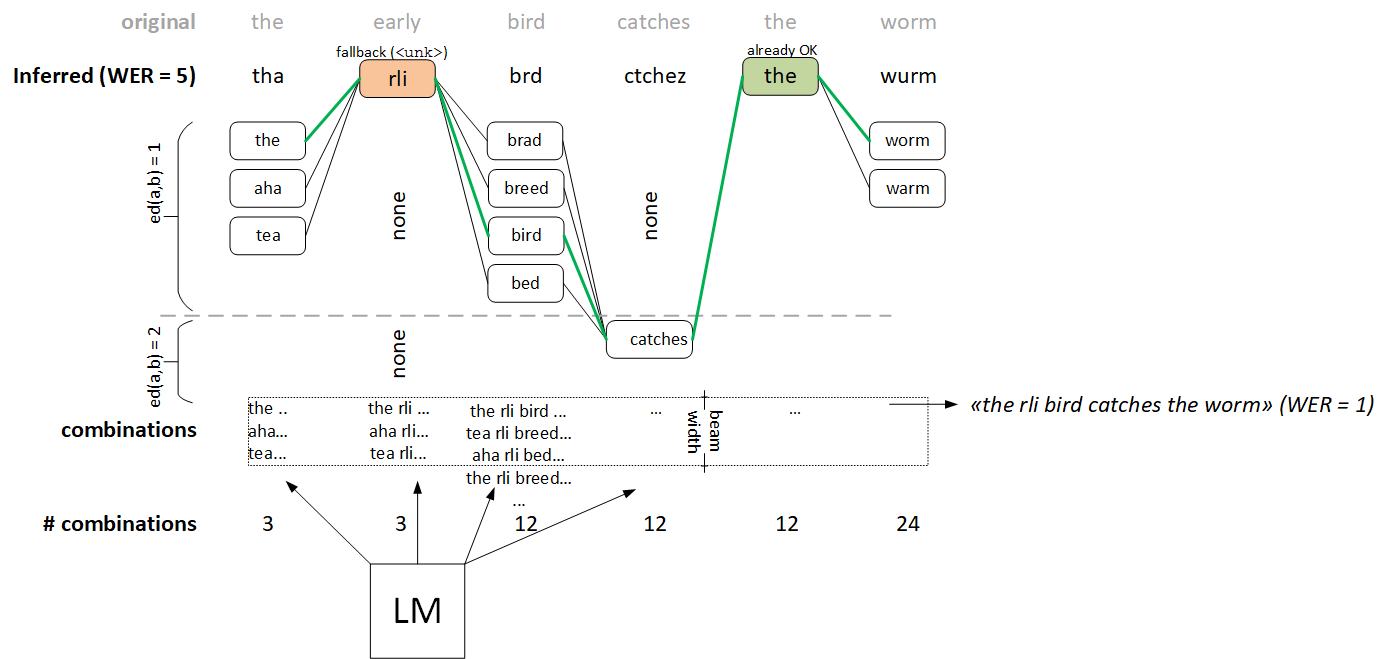
\includegraphics[width=\linewidth]{./img/spell_checker.png}
	\caption{Example of how the spell checker works}
	\label{spell-checker}
\end{figure}

A spell checker in combination with a \ac{LM} can help inferring orthographically correct words from sequences of characters inferred by \ac{CTC} and hence decrease the \ac{WER}. Therefore, by using a \ac{LM} the quality of transcriptions can improve considerably. Table \ref{ler_wer_example} illustrates this with an example.

\begin{table}[!htbp]
	\centering
	\begin{tabular}{llrrrr}
		\hline
		\thead{} &  & \thead{\ac{LER}} & \thead{\ac{LER}\\(norm.)} & \thead{\ac{WER}} & \thead{\ac{WER}\\(norm.)} \\
		\hline
		ground truth & i put the vice president in charge of mission control & $0$ & $0.00$ & $0$ & $0.00$ \\ 
		\hline
		before spell-checking & ii put he bice president in charge mission control & $6$ & $0.11$ & $4$ & $0.40$ \\ 
		\hline
		after spell-checking & i put the vice president in charge mission control & $3$ & $0.06$ & $1$ & $0.10$ \\
		\hline
	\end{tabular}
	\caption{Example for how a Spell-Checker (SC) can help improve the quality of an inferred transcription by changing characters and words. Audio and ground truth were taken from the \textit{ReadyLingua} corpus and the inference was made with the pre-trained \textit{DeepSpeech} model.}
	\label{ler_wer_example}
\end{table}

\subsubsection{Reducing the vocabulary size}

The \ac{LM} from Mozilla was trained on texts from the \textit{LibriSpeech} corpus\footnote{\url{http://www.openslr.org/11}}. Apart from lowercasing, the texts were not normalized or preprocessed. The resulting vocabulary is therefore very big and contains $973.673$ unique words. Because no further preprocessing was done, it also contains some exotic words like \textit{"zzzz"} and probably also misspelled words that happen to appear in the corpus. To train the \ac{LM}, $n$-grams of order 4 and 5 were pruned with a threshold value of 1, meaning only 4- and 5-grams with a minimum count of 2 and higher are estimated\footnote{see \url{https://github.com/mozilla/DeepSpeech/tree/master/data/lm}}. Because most spelling errors are probably unique within the training corpus, 4- or 5-grams containing an invalid word are unique too and most likely filtered out with pruning. 

Above procedure might work well to estimate the likelihood of a sentence. For a simple spell checker however, such a big vocabulary might be counter-productive because it lowers the probability that an obviously wrong word is corrected because for some reason it found its way into the vocabulary. Vice versa a very large vocabulary raises the probability that a random-looking sequence of characters is wrongfully exchanged with a (valid or invalid) word from the vocabulary. To prevent this, the original vocabulary was reduced into three vocabularies containing the $40.000$, $80.000$ and $160.000$ most frequent words from the corpus each. These words make up $98.42\%$, $99.29\%$ and $99.69\%$ of the corpus.

To create the vocabularies, a list of unique words and their frequency was created from the corpus and sorted by frequency in descending order. Naturally, stop words like \textit{the}, \textit{and} or \textit{of} appear at the top of the list. The first $40.000$, $80.000$ resp. $160.000$ words from this list were stored as the truncated vocabularies, the rest was discarded. Note that truncating the vocabulary only affects the way words are exchanged by the spell checker during post-processing, not how the likelihood of a post-processed sentence is estimated by the \ac{LM}.

\subsection{Further thoughts and considerations}

The spell checker in this project uses the vocabulary with $80.000$ words. This value was arbitrarily chosen and some unsystematic experiments were made to analyze the correctional capabilities of the spell checker. Because of time constraints and because it was unclear whether the spell checker would help improving the transcriptions in the first place, other vocabulary sizes were not evaluated. Further work may however try to find out an optimal vocabulary size for each language.

\subsection{Summary}

This chapter described how the $5$-gram \ac{LM} from the Mozilla implementation of \textit{DeepSpeech} was used to implement a rudimentary spell checker. This spell checker uses a vocabulary of the $80.000$ most frequent words from the corpus the \ac{LM} was trained on. It repeatedly swaps invalid words from an inferred transcript with valid words from the vocabulary and calculates the likelihood of various combinations of word sequences.